{
    \color{red}
    \begin{enumerate}
        \item Biological background
        \begin{enumerate}
            \item residue identity prediction
            \item atomic environments 
            \item SMILES representation?
        \end{enumerate}
        \item Machine learning background
        \begin{enumerate}
            \item neural networks
            \item graph neural networks
            \item equivariant graph neural networks
            \item representing residues as graphs
        \end{enumerate}
    \end{enumerate}
}

\section{Biological background}
\subsection{Proteins}
\textbf{Amino acids} are the building blocks of proteins and play a fundamental role in various biological processes. These small organic molecules are essential for life, and their unique properties allow them to form complex and diverse structures within the body. 
All amino acids follow the same underlying pattern and consist of a central carbon atom (C), an \textit{amino} group ($\text{NH}_3$), a \textit{carboxyl} group (COOH), and a variable side-chain, as we can see in Figure \ref{fig:amino-acid}.
Chains of amino acids are formed through a chemical reaction that creates a \textit{peptide bond}, as shown in Figure \ref{fig:residue}. The portions left of the original amino acids are called \textit{residues}. Note that there are 20 naturally occuring amino acids.
\begin{figure}
    \centering
    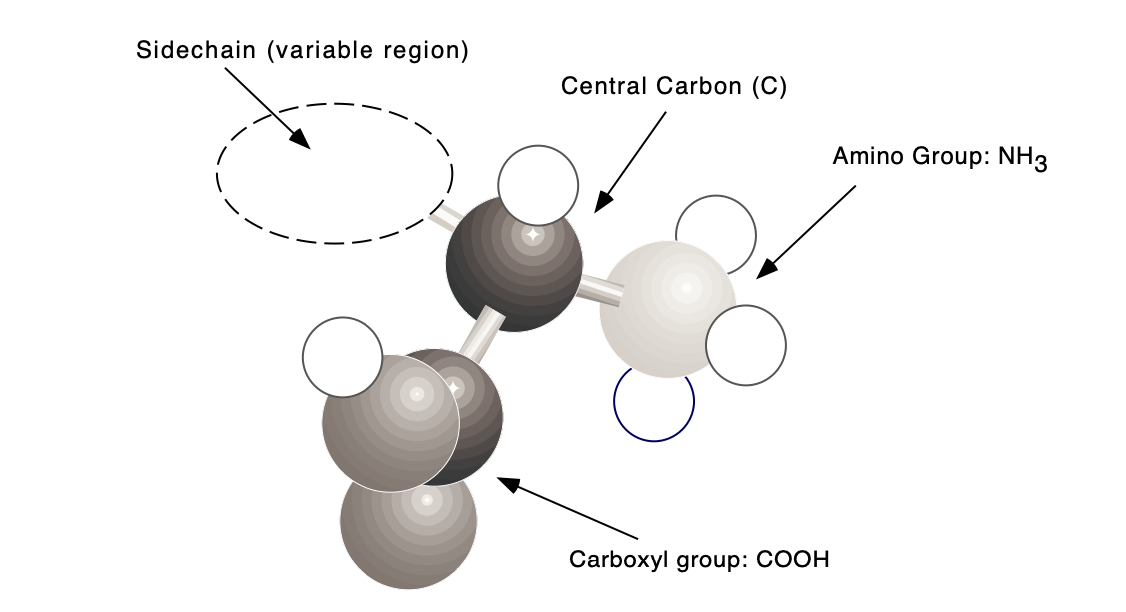
\includegraphics[scale=0.5]{figures/amino-acid.png}
    \caption{The basic chemical structure of an amino acid. Carbon atoms are black, Oxygen is dark grey, Nitrogen light grey, and hydrogen white. Image taken from \cite{hunter1993molecular}.}
    \label{fig:amino-acid}
\end{figure}

\begin{figure}
    \centering
    \begin{tikzpicture}
    \node (acidone) {\chemfig[atom sep=2em]{N(-[3]H)(-[5]H)-C(-[2]H)(-[6]R_1)-C(-[1]{\color{blue}OH})(=[7]O)}};
    \node[right of=acidone, xshift=3cm] (acidtwo) {\chemfig[atom sep=2em]{N(-[3]H)(-[5]{\color{blue}H})-C(-[2]H)(-[6]R_2)-C(-[1]OH)(=[7]O)}};
    \draw[->,thick] ($(acidone.east)!0.5!(acidtwo.west)$) ++(0, -1.2cm) -- ++(0,-0.8cm) node[right] {};
    \node[below of=acidone, xshift=2cm, yshift=-2.4cm] (residue) 
        {\chemfig[atom sep=2em]{N(-[3]H)(-[5]H)-C(-[2]H)(-[6]R_1)-C(=[7]O)-[1,,,,blue]N(-[3]H)-C(-[2]H)(-[6]R_2)-C(=[7]O)(-[1]OH)}};
    
    \node[below of=residue, yshift=-0.7cm, xshift=-1.5cm] (res1) {\textit{residue 1}};
    \node[below of=residue, yshift=-0.7cm, xshift=1.5cm] (res1) {\textit{residue 2}};
    \end{tikzpicture}
    \caption{Two amino-acids are chained together through a peptide bond. The chemical reaction releases a water molecule ($\text{H}_2\text{O}$) in the process.}
    \label{fig:residue}
\end{figure}
\textbf{Proteins} are one of the most important macromolecules found in living organisms and they are involved in a vast array of biological processes. 
These large, complex molecules are composed of long chains of amino acids that are folded into shapes.
Proteins play a variety of roles in the body, including catalysing chemical reactions, transporting molecules, providing structural support, and regulating gene expression. 
The diversity of protein structures and functions is vast, with some proteins consisting of just a few amino acids, while others contain thousands. 
The unique sequence of amino acids in each protein determines its three-dimensional structure and, more importantly, its \textit{specific function}. 
Understanding the structure and function of proteins is essential for advancing our knowledge of cellular processes and for developing treatments for a range of diseases caused by protein dysfunction.
\subsection{Residue identity prediction}
Residue identity prediction (RES) is a computational task in bioinformatics that involves predicting the amino acid residue at a particular position within a protein sequence. 
The accurate prediction of residue identity is an important problem in bioinformatics because it can provide insights into protein function, structure, and evolution. 
Knowing the identity of residues within a protein sequence can help to identify important functional sites and motifs, which can provide clues about the protein's function and interactions with other molecules. 

Residue identity prediction is also important for \textit{protein engineering}, as it can help researchers design proteins with specific functions.
Machine learning approaches to RES have already been used to engineer plastic decomposing enzymes for higher thermal stability \cite{Lu2022}.

\paragraph{The ATOM3D dataset.} One important benchmark dataset for RES is ATOM3D \cite{atom-3d}.
The ATOM3D collection is a compilation of datasets that contain the 3D structure of biomolecules, including nucleic acids, small molecules, and proteins. 
These datasets have been tailored to function as a benchmark for machine learning techniques that train on the 3D molecular structure of molecules in order to solve tasks such as molecular function prediction, ligand binding affinity, or protein-protein interactions.

\paragraph{The PDB format.} ATOM3D datasets have a standardised format, in which each sample is a \texttt{.pdb} file. The \texttt{.pdb} format is a format provided by the \textbf{Protein Data Bank} (PDB), a database of 3D structural data of various biological molecules. Figure \ref{pdb} shows an example of a molecule from the PDB.
\begin{figure}
    \centering
    \subfigure[The 1KDA molecule. The orange structure represents one amino acid residue.]{
        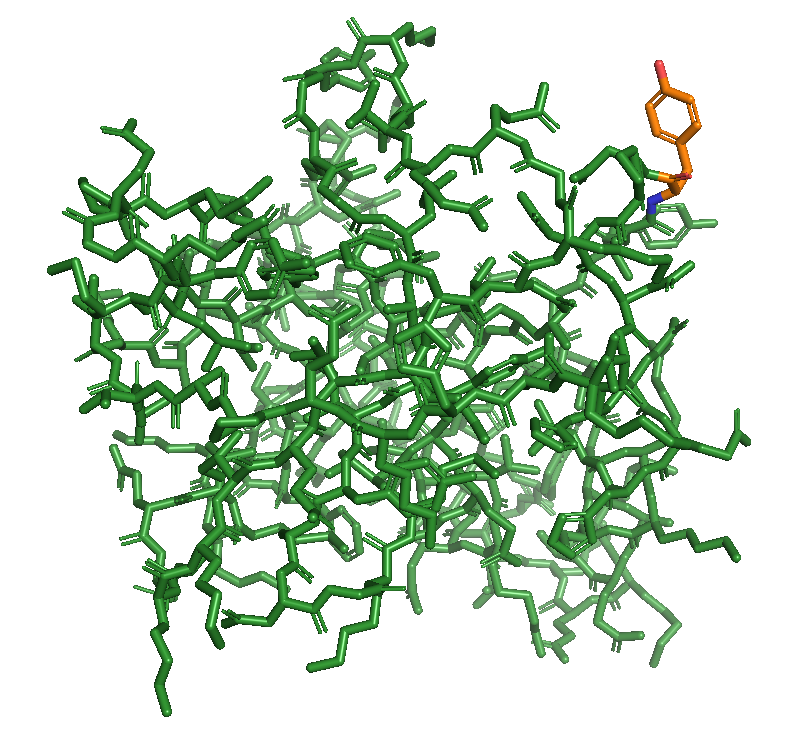
\includegraphics[scale=0.15]{figures/1kda_example.png}
    }
    \hspace{0.3in}
    \subfigure[A close-up of the atomic environment around the orage amino-acid.]{
        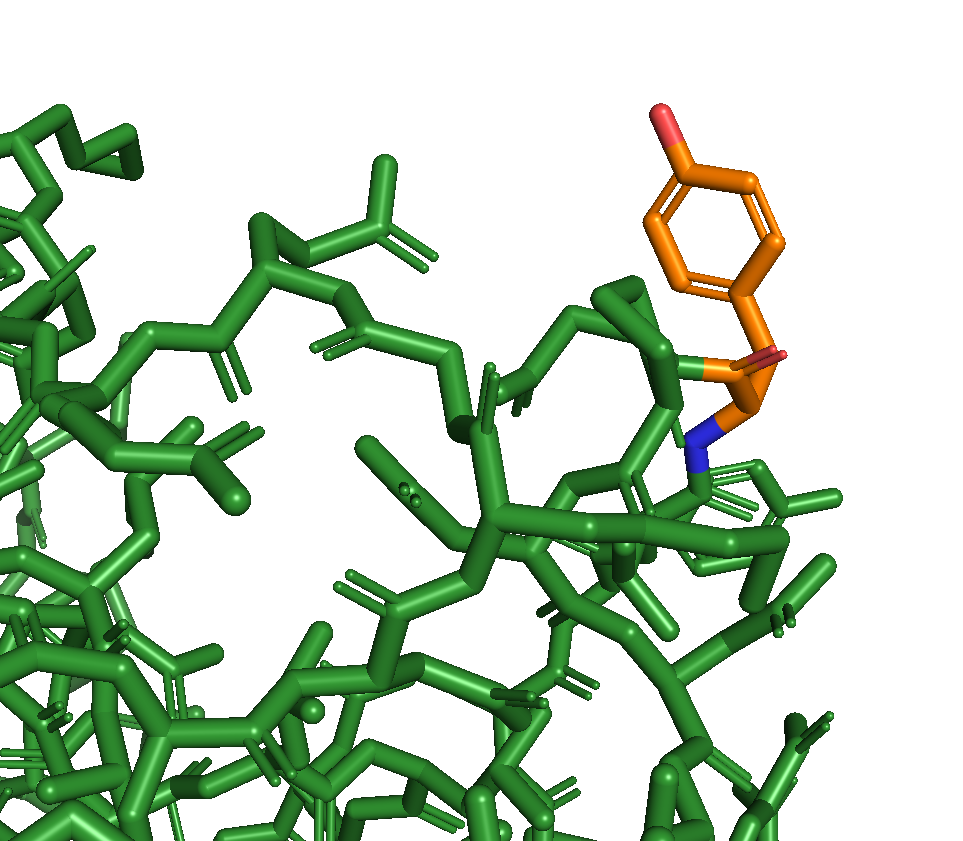
\includegraphics[scale=0.15]{figures/1kda_closeup.png}
    }
    
    \caption{Example of a PDB molecule.}
    \label{pdb}
\end{figure}
\section{Machine learning background}
\subsection{Graph Neural Networks}
\subsection{Equivariant Graph Neural Networks}
\subsection{Representing residues as graphs}
